\documentclass[10pt]{ctexart}
\usepackage{graphicx, amsmath}
\usepackage{siunitx}
\usepackage{caption}
\usepackage{url}
\usepackage[version=4]{mhchem}
\title{康普顿散射实验}
\author{张爱强\\指导教师: }
\date{}
% set the section title format
\ctexset{
    section/format  += \raggedright
}
% The following parameters seem to provide a reasonable page setup.
\topmargin 0.0cm
\oddsidemargin 0.2cm
\textwidth 16cm 
\textheight 21cm
\footskip 1.0cm
% set the abstract format
\newenvironment{sciabstract}{%
\begin{quote} \textbf{摘要: }}
{\end{quote}}
% set the bibliography format
\bibliographystyle{elsarticle-num}


\begin{document}
\maketitle
\begin{sciabstract}
    本实验利用非热光源作为成像光源,分别使用桶探测器和面探测器对物体进行成像,将成像结果做对应的操作,可以获得物体的成像结果。本实验验证了量子关联成像
    的结果。
    \par\textbf{关键词: } 量子关联成像.
\end{sciabstract}
\section{引言}
量子关联成像是一种特殊的非直接成像方式,利用光场的二阶乃至高阶关联性质,间接重构出
图像\cite{pkuWeb}。将光源通过分束器分成两路,一路经过物体后用
没有空间分辨率的桶探测器收集,另外一路不与物体接触,由面探测器收集。两路结果通过关联计算重构出物体图像。
\section{实验}
实验装置图如图~\ref{fig:instrument}所示
\begin{figure}
    \centering
    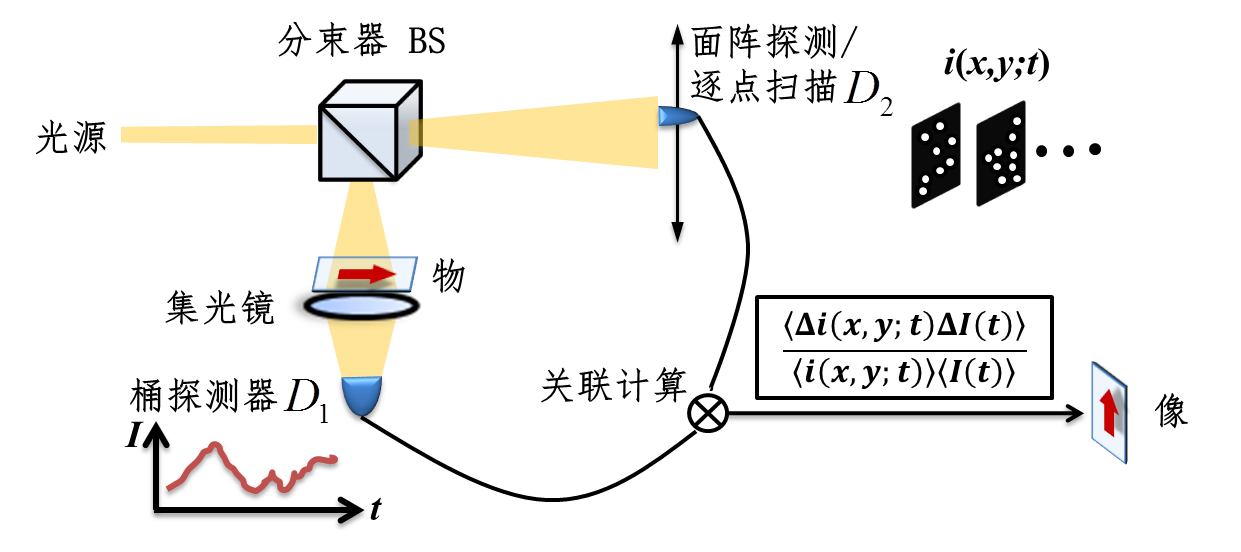
\includegraphics[width=0.8\textwidth]{data/instrument.png}
    \caption{量子关联成像装置图}
    \label{fig:instrument}
\end{figure}
\section{结果}
实验结果得到的成像为图~\ref{fig:picture},其中桶探测器某一帧的成像为
图~\ref{fig:pic1},面探测器为图~\ref{fig:pic2}。
\begin{figure}
    \centering
    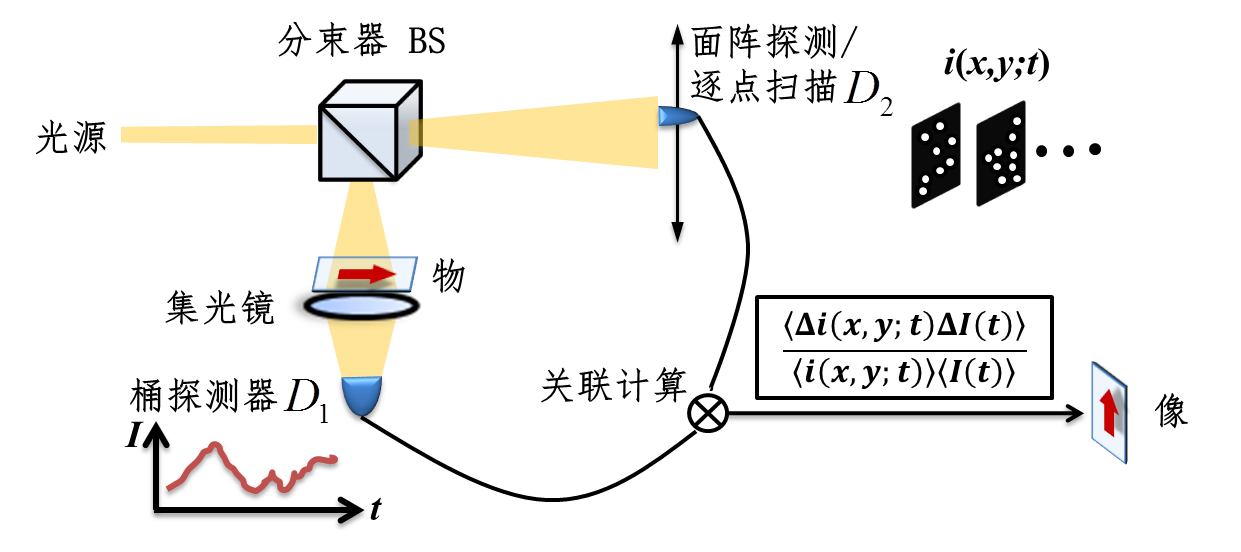
\includegraphics[width=0.8\textwidth]{data/instrument.png}
    \caption{量子关联成像图}
    \label{fig:picture}
\end{figure}
\begin{figure}
    \centering
    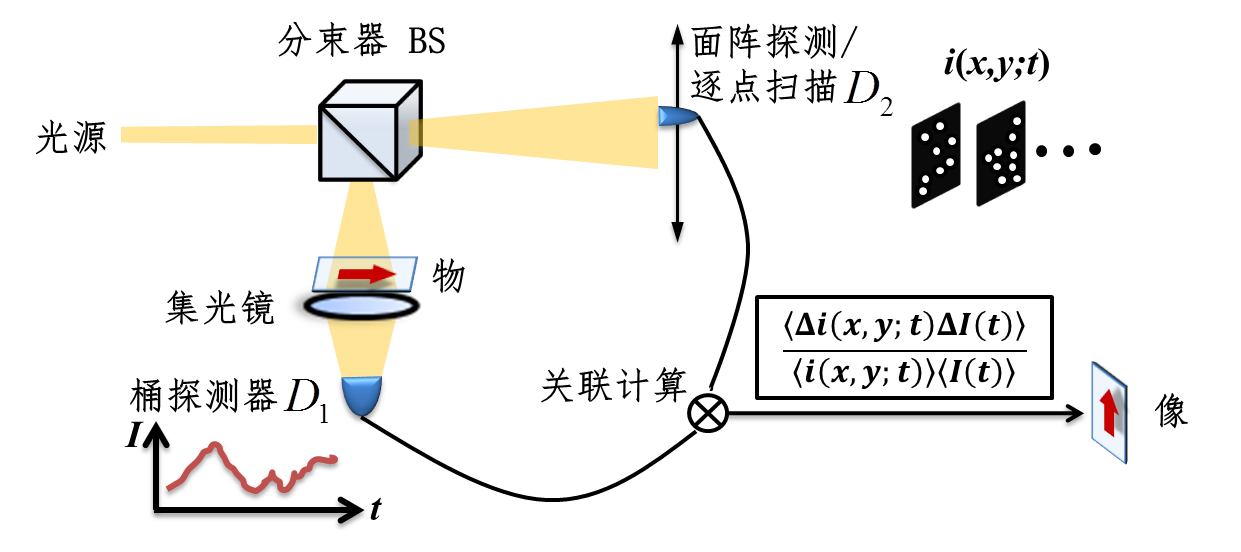
\includegraphics[width=0.8\textwidth]{data/instrument.png}
    \caption{桶探测器图像}
    \label{fig:pic1}
\end{figure}
\begin{figure}
    \centering
    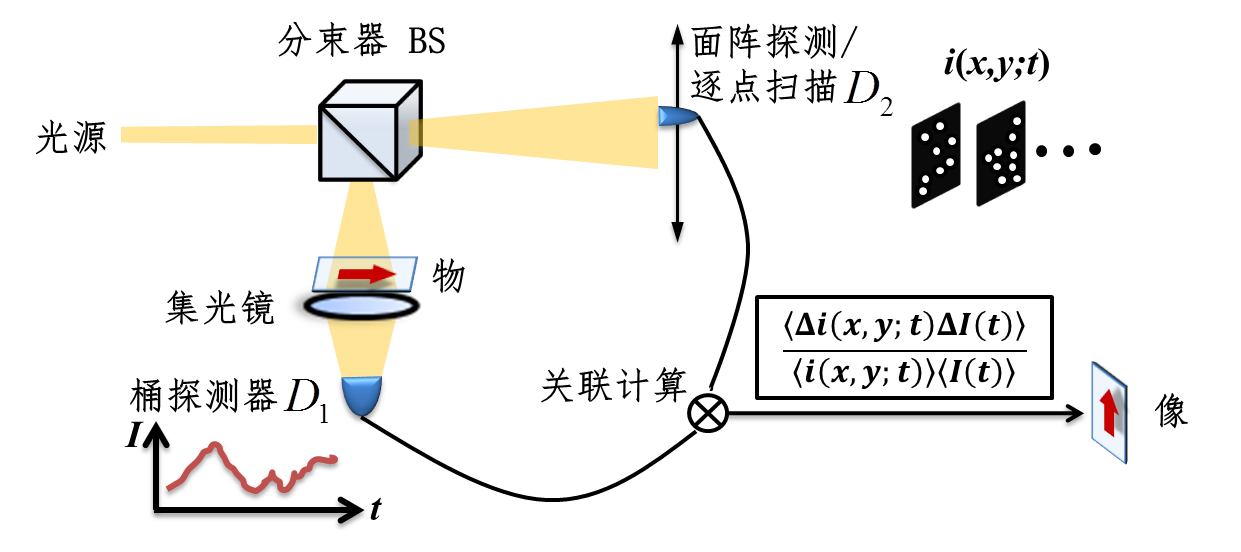
\includegraphics[width=0.8\textwidth]{data/instrument.png}
    \caption{面探测器图像}
    \label{fig:pic2}
\end{figure}
\section{结论}
\bibliography{report}
\end{document}